% Based on the template from Pandoc 3.1.11.1. Custom sections are marked 'CUSTOM'.
% Customisations go in included files where possible, but this isn't always
% possible.
% Options for packages loaded elsewhere
\PassOptionsToPackage{unicode}{hyperref}
\PassOptionsToPackage{hyphens}{url}
\PassOptionsToPackage{dvipsnames,svgnames,x11names}{xcolor}
%
\documentclass[
  12pt,
  a4paper,
]{article}
\usepackage{amsmath,amssymb}
\usepackage{iftex}
\ifPDFTeX
  \usepackage[T1]{fontenc}
  \usepackage[utf8]{inputenc}
  \usepackage{textcomp} % provide euro and other symbols
\else % if luatex or xetex
  \usepackage{unicode-math} % this also loads fontspec
  \defaultfontfeatures{Scale=MatchLowercase}
  \defaultfontfeatures[\rmfamily]{Ligatures=TeX,Scale=1}
\fi
\usepackage{lmodern}
\ifPDFTeX\else
  % xetex/luatex font selection
  \setmainfont[]{TeX Gyre Termes}
\fi
% Use upquote if available, for straight quotes in verbatim environments
\IfFileExists{upquote.sty}{\usepackage{upquote}}{}
\IfFileExists{microtype.sty}{% use microtype if available
  \usepackage[]{microtype}
  \UseMicrotypeSet[protrusion]{basicmath} % disable protrusion for tt fonts
}{}
\usepackage{fancyvrb}
\usepackage{xcolor}
\usepackage[a4paper]{geometry}
\usepackage{graphicx}
\makeatletter
\def\maxwidth{\ifdim\Gin@nat@width>\linewidth\linewidth\else\Gin@nat@width\fi}
\def\maxheight{\ifdim\Gin@nat@height>\textheight\textheight\else\Gin@nat@height\fi}
\makeatother
% Scale images if necessary, so that they will not overflow the page
% margins by default, and it is still possible to overwrite the defaults
% using explicit options in \includegraphics[width, height, ...]{}
\setkeys{Gin}{width=\maxwidth,height=\maxheight,keepaspectratio}
% Set default figure placement to htbp
\makeatletter
\def\fps@figure{htbp}
\makeatother
\ifLuaTeX
  \usepackage{luacolor}
  \usepackage[soul]{lua-ul}
\else
  \usepackage{soul}
\fi
\setlength{\emergencystretch}{3em} % prevent overfull lines
\providecommand{\tightlist}{%
  \setlength{\itemsep}{0pt}\setlength{\parskip}{0pt}}
\setcounter{secnumdepth}{-\maxdimen} % remove section numbering
\ifLuaTeX
\usepackage[bidi=basic]{babel}
\else
\usepackage[bidi=default]{babel}
\fi
\babelprovide[main,import]{british}
\ifPDFTeX
\else
\babelfont{rm}[]{TeX Gyre Termes}
\fi
% get rid of language-specific shorthands (see #6817):
\let\LanguageShortHands\languageshorthands
\def\languageshorthands#1{}
\usepackage{bold-extra}
\usepackage[perpage,symbol*]{footmisc}
\usepackage[labelformat=empty]{caption}

\usepackage{titlesec}

\special{pdf:trailerid [
    <72af687631737750e85ffac90f246dcf>
    <72af687631737750e85ffac90f246dcf>
]}
\ifLuaTeX
  \usepackage{selnolig}  % disable illegal ligatures
\fi
\usepackage{bookmark}
\IfFileExists{xurl.sty}{\usepackage{xurl}}{} % add URL line breaks if available
\urlstyle{same}
\VerbatimFootnotes % allow verbatim text in footnotes
\hypersetup{
  pdftitle={The Title},
  pdfauthor={An Author},
  pdflang={en-GB},
  pdfsubject={Version: reproducible},
  colorlinks=true,
  linkcolor={black},
  filecolor={Maroon},
  citecolor={Blue},
  urlcolor={Blue},
  pdfcreator={LaTeX via pandoc}}

\title{The Title}
\author{An Author}
\date{}

\begin{document}
\maketitle

\frenchspacing

\newcommand{\sectionbreak}{\clearpage}

\makeatletter
\@afterindentfalse
\@afterheading
\makeatother

This is some text before a section. It shouldn't be indented. Each
section should start on a new page (but subsections shouldn't).

\section{This is a section}\label{__h1_1}

\makeatletter
\@afterindentfalse
\@afterheading
\makeatother

This is some test text. This is formatted in \emph{italics} and
\textbf{bold}, with - various -- dashes---, and trailing dots\ldots{}

`These quotes should be curly,' and ``so should these.'' There should be
a blank line before the next paragraph:

~

\makeatletter
\@afterindentfalse
\@afterheading
\makeatother

And then there should be some text \textsuperscript{in~superscript} and
\textsubscript{in~subscript}, and a footnote\footnote{This is a
  footnote. It should appear at the bottom of the page.} with a star, a
footnote\footnote{Another footnote.} with a dagger, and this should be
\texttt{monospace}.

\subsection{Subsection}\label{__h2_1}

\makeatletter
\@afterindentfalse
\@afterheading
\makeatother

Test text test text test text.

\begin{quote}
This is a quote block. It should be indented slightly and shouldn't
contain a line break.
\end{quote}

\begin{quote}
This is a quoted line block. It should be indented slightly\\
and have a \emph{line break} after `slightly', and \textbf{formatting}.
\end{quote}

\begin{quote}
``These literal double curly quotes, used where smart\\
quotes gets it wrong, curl the right way even though\\
they're on different lines.''
\end{quote}

\begin{quote}
`These literal single curly quotes, used where smart\\
quotes gets it wrong, curl the right way even though\\
they're on different lines.'
\end{quote}

\makeatletter
\@afterindentfalse
\@afterheading
\makeatother

After this line there should be stars.

\begin{center}* * *\end{center}

\makeatletter
\@afterindentfalse
\@afterheading
\makeatother

This is a new paragraph after the stars. This text is \textsc{Small
Caps}. Here is a pound sign (£), a euro sign (€), and three letters with
accents: ëóû.

\section{This is a second section}\label{__h1_2}

\begin{figure}
\centering
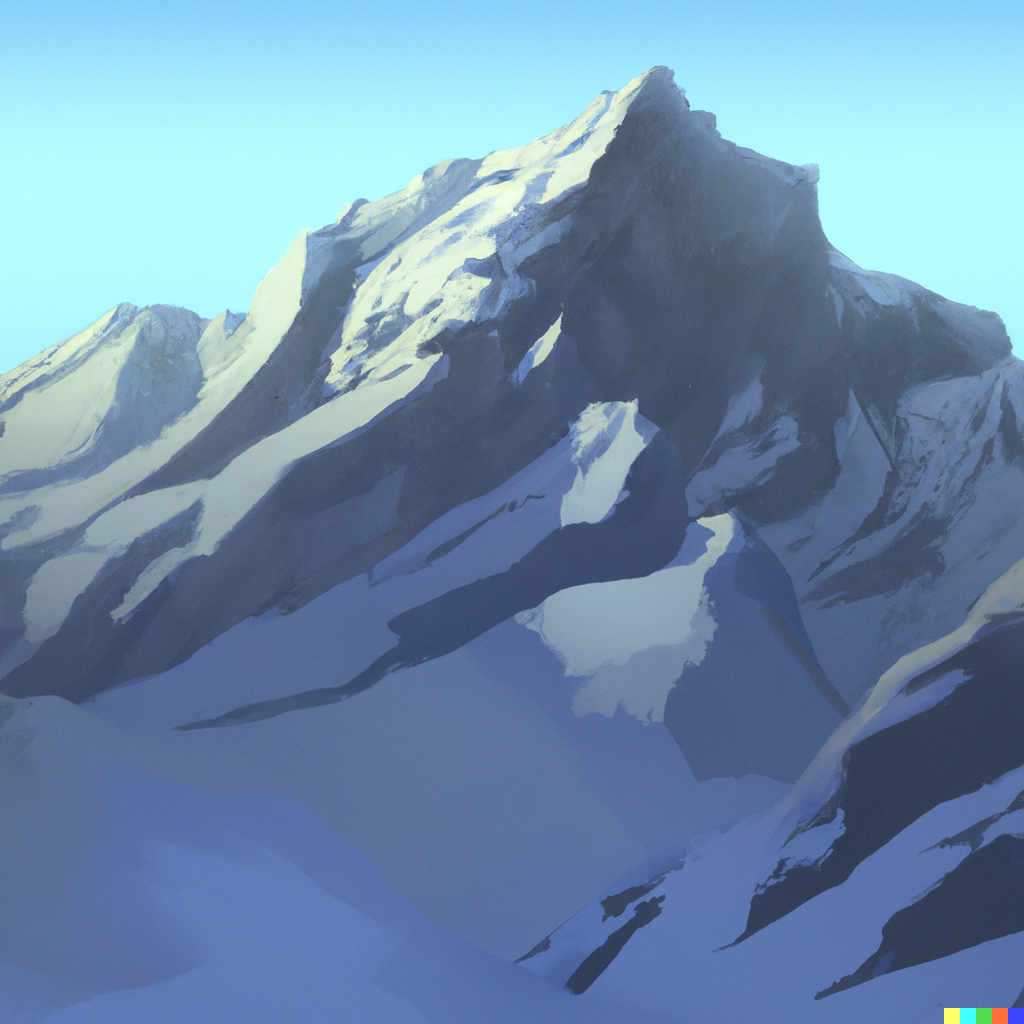
\includegraphics[width=0.5\textwidth,height=\textheight]{tests/test2/image.jpg}
\caption{foo}
\end{figure}

\makeatletter
\@afterindentfalse
\@afterheading
\makeatother

There is an image here.

And this is \emph{even more italic text}.

\end{document}
